

Using  SSL to authenticate  clients and  to protect  the communication
between client and target requires no changes in your source code. The
only  notable  effect  is  that  SSL/TLS type  sockets  are  used  for
transport  connections  instead of  plain  TCP  sockets  --- and  that
connection setup takes a bit longer.

The only  prerequisites are that you rebuild  JacORB with cryptography
support. You  also need  to set up  a key  store file that  holds your
cryptographic   keys,  and  to   configure  SSL   by  setting   a  few
properties. All of this is described in this chapter.

\section{Re--Building JacORB's security libraries}

In the  standard distribution, the  JacORB security libraries  are not
enabled.   To do  so, you  simply need  to recompile  JacORB  with the
required SSL libraries  in your CLASSPATH.  If these libraries
are not found, JacORB will be rebuilt without SSL support.

To  successfully rebuild  JacORB with  SSL support,  the  following is
required:

\begin{itemize}
        \item when using IAIKs libraries:
              \begin{itemize}
                \item IAIK-JCE 2.591 or later, the security provider classes
                downloadable from \\ \href{http://jcewww.iaik.tu-graz.ac.at}{http://jcewww.iaik.tu-graz.ac.at},
              \item iSaSiLk 3.0 or later, the SSL implementation from the same
                source.
              \end{itemize}

        \item when using Suns libraries:
              \begin{itemize}
              \item JDK 1.4 or JSSE 1.0.3 or above available from the
                Sun's Java Webpages (for JSSE 1.0.3, please see the
                {\tt README.jsse\_1\_0\_3} in
                {\tt src/org/jacorb/security/ssl/sun\_jsse} on how to compile).
              \item For key management, you also need additional packages like
                OpenSSL. These are not necessary for JacORB to work.
              \end{itemize}
\end{itemize}

Install the desired packages and read the documentation carefully. After
successfull installation, build JacORB anew by typing {\tt ant} in your JacORB
installation directory.


\section{Key stores}

SSL  relies   on  public  key  certificates  in   the  standard  X.509
format. These  certificates are presented in  the authentication phase
of the  SSL handshake and used  to compute and  exchange session keys.

The Java 2  security API provides interfaces that  access a persistent
data structure  called {\em  KeyStore}. A key  store is simply  a file
that contains  public key  certificates and the  corresponding private
keys. It also  contains other certificates that can  be used to verify
public key  certificates.  All  cryptographic data is  protected using
passwords and accessed using names called {\em aliases}.

The following section explain how to create key stores for Sun JSSE
and for IAIK.

%Note that  key  stores  are normally  used  only for  client
%authentication in JacORB.   Servers may, but need not,  have their own
%keys and  passwords because server authentication is  optional and not
%mandatory like  client authentication. Technically,  this is achieved
%by  exchanging the  client  and server  roles  at SSL  setup. This  is
%entirely  transparent to  applications, of  course, but  might prevent
%interoperation  with other ORBs  over SSL  if their  SSL setup  is not
%prepared to handle this role change.

\subsection{Setting up a JSSE key store}

To set up key stores with JSSE you can use Java's {\tt keytool}.
In  order to  generate  a  simple public  key  infrastructure you  can
perform the following steps:

\begin{enumerate}
\item Create a new key store containing a new public/private key pair
with {\tt keytool}. The public key will be wrapped into a self-signed certificate.
\item Export the self-signed certificate from the key store into a file.
\item Import the self-signed certificate into a trust store
   (or configure that trustees shall be read from key store, see below).
\end{enumerate}
To create a new key store containing a new public/private key pair type:
\begin{verbatim}
   keytool -genkey -alias <alias> -keystore <keystore>
\end{verbatim}
If you don't give a key store name {\tt keytool} will create a key store with
the name {\tt .keystore} in the user's home directory. The command
given above will ask for the following input:
\begin{verbatim}
   Enter keystore password:  changeit
   What is your first and last name?
     [Unknown]:  Developer
   What is the name of your organizational unit?
     [Unknown]:  cs
   What is the name of your organization?
     [Unknown]:  PrismTech
   What is the name of your City or Locality?
     [Unknown]:  Berlin
   What is the name of your State or Province?
     [Unknown]:  Berlin
   What is the two-letter country code for this unit?
     [Unknown]:  Germany
   Is CN=Developer, OU=cs, O=PrismTech, L=Berlin, ST=Berlin,
      C=Germany correct?
     [no]:  yes

   Enter key password for <testkey>
        (RETURN if same as keystore password):  testkey
\end{verbatim}
You can view the entries of the newly created keystore by typing:
\begin{verbatim}
keytool -keystore <keystore> -list -storepass <password>
\end{verbatim}
The output will read for example like this:

\begin{verbatim}
   Keystore type: jks
   Keystore provider: SUN

   Your keystore contains 1 entry

   testkey, Dec 1, 2004, keyEntry,
   Certificate fingerprint (MD5): C4:9B:11:97:FF:CD:4C:C9:B3:02:BB:
   9A:46:D8:C3:11
\end{verbatim}

Now you have a public key certificate that you can present for
authentication. The public key contained in the key store is wrapped
into a self-signed certificate. This self-signed certificate has to be
added to the Java trust store. To do this export the certificate from
the key store and import it into the Java trust store located in {\tt
<java\_home>/jre/lib/security/cacerts}.

To export the self-signed certificate into a file type:
\begin{verbatim}
keytool -export -keystore <keystore> -alias <alias> -file <filename>
\end{verbatim}
To import the certificate into the trust store type:
\begin{verbatim}
keytool -import -keystore <truststore> -alias <alias> -file <filename>
\end{verbatim}

More documentation on key stores  can be found in the Java tool
documentation for the {\tt keytool}  command. Note that if you care
for ``real'' security,  be advised  that setting  up  and managing
(or finding)  a properly administered CA is essential for the overall
security of your system.

%\section{IAIK specific setup}
%This section covers topics that are specific to IAIKs libraries.

\subsection{Setting up an IAIK key store}

JacORB provides a  GUI tool to create and  manipulate IAIK key store
files, the  KeyStoreManager. It  can generate  key pairs,  sign
public keys, import  or   export  certificates,  and   define  trusted
certificate authorities. To start the KeyStoreManager, simply type
{\tt ks} on the command  line. The GUI  lets you  select and  open
existing  key store files, or create new ones.

Starting with an  empty key store, you first need to  create a new key
store and then  a key pair and certificate. Select  {\tt New} from the
{\tt File}  menu to create  a key store,  and then {\tt New}  from the
{\tt Keys} menu.   You will then be asked to provide  a new alias name
for your  new key entry. You also  need to choose a  password. You can
leave  the  algorithm  and  key  length fields  in  the  combobox  menu
unchanged.

\bigskip
\begin{center}
  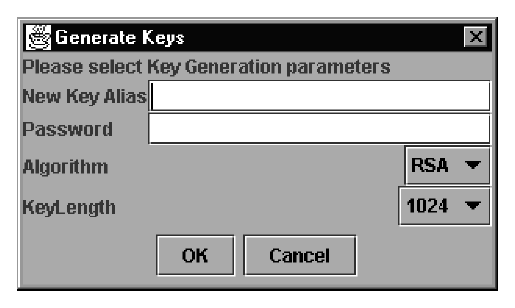
\includegraphics[width=7cm]{SSL/Generate}
\end{center}

You  now  have a  public  key certificate  that  you  can present  for
authentication, claiming  identity with the  alias name that  has been
embedded  in the  certificate.   Since anybody  could  present such  a
certificate,  receivers  require  that  the certificate  be  digitally
signed by someone  they trust, a {\em Certificate  Authority} (CA). By
signing  the certificate,  a CA  supports  the identity  claim of  the
certificate  subject. Whose  signature is  accepted as  trustworthy is
just a matter  of configuration, but normally proper  CAs are expected
to only sign certificates that  they have carefully scrutinized --- or
even created themselves.

\bigskip
\centerline{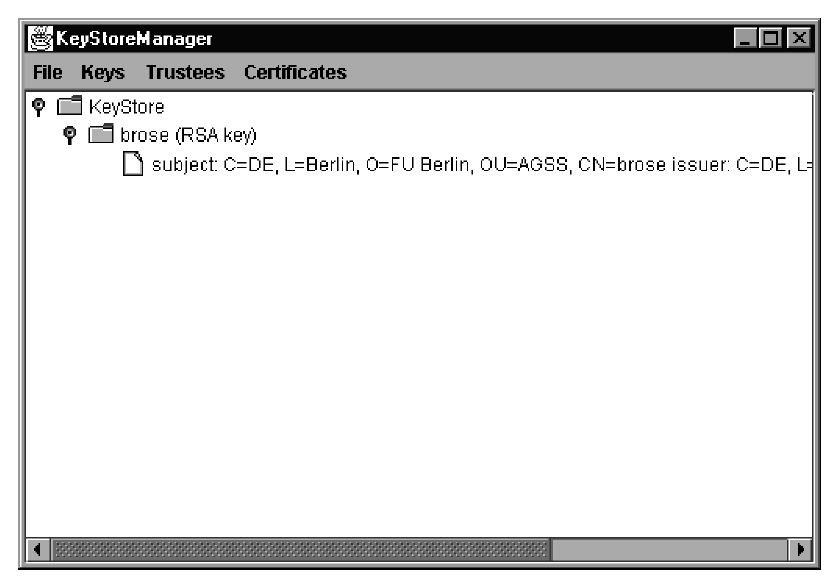
\includegraphics[width=11cm]{SSL/Keystore}}

For   convenience  you   can  act   as  a   CA  yourself,   using  the
KeyStoreManager GUI  to import certificates  and then sign  and export
them  again.   The  originating  key  store can  then  re--import  the
certificate that now bears the  digital signature of someone acting as
a CA. The key store has a  standard key chain format that must be used
to store public key certificates. The  first entry in the key chain is
your own public  key certificate as generated by the  key store. It is
automatically signed with its own  private key. Second in the chain is
the public key certificate that is signed by the CA. The last entry in
a key  chain must hold the  CA's public key  certificate, signed using
its private key. Trust in the CA key is ``axiomatic''.

\bigskip
\centerline{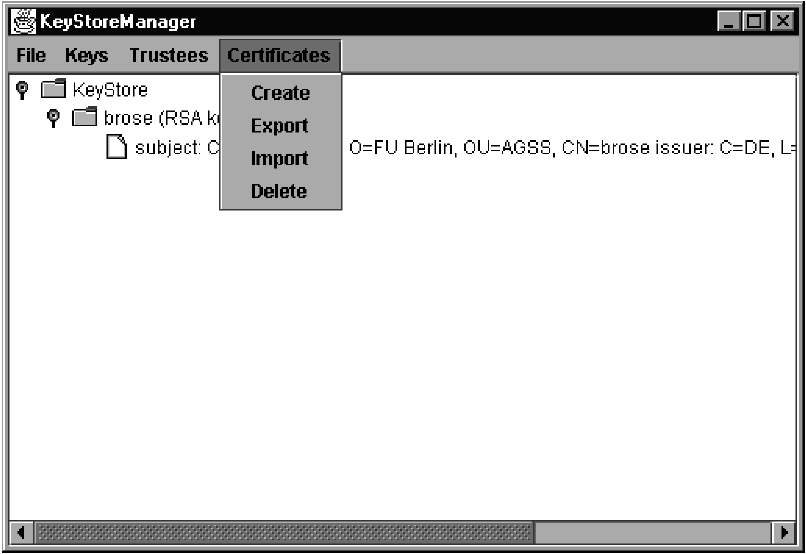
\includegraphics[width=11cm]{SSL/KSMenu}}

You can  check the validity of a  key chain by selecting  an alias and
then choosing {\tt Verify Chain}  from the {\tt Keys} menu. Unless the
key  chain  has  the proper  format  {\em  and}  the CA's  public  key
certificate is also declared  as trusted using the {\tt Trustees--add}
menu, the  verification will fail.  Only of  the verification succeeds
will you be able to use a public key certificate in the SSL connection
setup.

\subsection{Step--By--Step certificate creation}
In  order to  generate  a  simple public  key  infrastructure you  can
perform the following steps:
\begin{enumerate}
\item Create new key stores (File/new) and keypairs (Keys/new) for the CA
and for the user.
\item  Open the  user keys tore (File/open),  select the  key  entry and
export the self-signed certificate (Certificates/Export).
\item  Open  the  CA  key store  and  add the  user  certificate  as  a
Trustee (Trustees/add\dots).
\item Select the  trusted user certificate and create  a signed public
key certificate (Certificates/Create). Leave the role name field empty,
enter the  CAs private  key password and  save the new  certificate by
clicking OK.
\item Export the  CAs self-signed certificate to a  file (as explained
above).    Delete    the    trusted    certificate   from    the    CA
key store (Trustees/Delete).
\item Open the  user key store again. Select the  key entry, the import
the CA-signed  user cert (Certificates/Import), and  the self-signed CA
cert.
\item Add  the self-signed CA cert  as a trustee. This  is only needed
for verifying the chain, therefor the key store can be deployed without
it.  Please  note  that  a  failed  verification  might  result  in  a
SignatureException.
\end{enumerate}

\section{Configuring SSL properties}

When the ORB is initialized by the application, a couple of properties
are read from files and the  command line. To turn on SSL support, you have to
set the following property to ``on'':

\begin{verbatim}
        jacorb.security.support_ssl=on
\end{verbatim}

This will just load the SSL classes on startup. The configuration of the
various aspects of SSL is done via additional properties.

Configure which SSL socket factory and SSL server socket factory shall
be used with the properties:
\begin{verbatim}
         jacorb.ssl.socket_factory=qualified classname
         jacorb.ssl.server_socket_factory=qualified classname
\end{verbatim}

If you want to use JSSE, then configure the following as qualified
classname of SSL Socket Factory and SSL server socket factory:
\begin{verbatim}
         org.jacorb.security.ssl.sun_jsse.SSLSocketFactory
         org.jacorb.security.ssl.sun_jsse.SSLServerSocketFactory
\end{verbatim}
%jacorb.ssl.server_socket_factory=org.jacorb.security.ssl.sun_jsse.SSLSocketFactory

If you want to use IAIK, then configure the following as qualified
classname of SSL Socket Factory and SSL server socket factory:
\begin{verbatim}
         org.jacorb.security.ssl.iaik.SSLSocketFactory
         org.jacorb.security.ssl.iaik.SSLServerSocketFactory
\end{verbatim}
%jacorb.ssl.server_socket_factory=org.jacorb.security.ssl.iaik.SSLSocketFactory

As explained  in the previous  section, cryptographic data  (key pairs
and  certificates) is  stored in  a  key store  file. To configure the
file name of the key store file, you need to define the following
property:

\begin{verbatim}
        jacorb.security.keystore=AKeystoreFileName
\end{verbatim}

The key store file name can either be an absolute path or relative to
the home directory. Key stores are searched in this order, and the
first one found is taken. If this property is not set, the user will be
prompted to enter a key store location on ORB startup.

To avoid  typing in  lots of  aliases and passwords  (one for  the key
store, and  one for each entry  that is used), you  can define default
aliases and passwords like this (the default user only applies when
using IAIK):

\begin{verbatim}
# the name of the default key alias to look up in the key store
jacorb.security.default_user=brose
jacorb.security.default_password=jacorb
\end{verbatim}

Note that when using Sun JSSE: The {\tt javax.net.ssl.trustStore[Password]}
properties doesn't seem to take effect, so you may want to add trusted
certificates to "normal" key stores. In this case configure JacORB to read
certificates from the key store rather than from a dedicated trust
store, please set the property
\begin{verbatim}
jacorb.security.jsse.trustees_from_ks=on
\end{verbatim}

SSL settings can be further refined using security options as in
the following property definitions:

\begin{verbatim}
        jacorb.security.ssl.client.supported_options=0
        jacorb.security.ssl.client.required_options=0

        jacorb.security.ssl.server.supported_options=0
        jacorb.security.ssl.server.required_options=0
\end{verbatim}

The  value  of  these security  options  is  a  bit  mask coded  as  a
hexadecimal integer. The meanings of the individual bits is defined in
the CORBA Security Service  Specification and reproduced here from the
{\tt Security.idl} file:

\begin{verbatim}
        typedef unsigned short   AssociationOptions;

        const AssociationOptions NoProtection = 1;
        const AssociationOptions Integrity = 2;
        const AssociationOptions Confidentiality = 4;
        const AssociationOptions DetectReplay = 8;
        const AssociationOptions DetectMisordering = 16;
        const AssociationOptions EstablishTrustInTarget = 32;
        const AssociationOptions EstablishTrustInClient = 64;
        const AssociationOptions NoDelegation = 128;
        const AssociationOptions SimpleDelegation = 256;
        const AssociationOptions CompositeDelegation = 512;
\end{verbatim}

% With the current SSL integration in JacORB, the only valid settings
% are EstablishTrustInTarget and/or EstablishTrustInClient, i.e.  hex
% values 20, 40 or 60. NoProtection is not possible when SSL is used. If
% you don't want protection, switch SSL support off. The following
% sections go into some more detail about what specific property values
% mean.

\subsection{Client side and server side configuration}
On both the client side and the server side supported and required
options can be configured. The following tables explain the settings
for supported and required options for client and server.

\begin{table}
\caption{Client side supported options}
\begin{tabular}{|p{7cm}|p{7cm}|}
\hline
\textbf{Property with value}& \textbf{Description}\\
\hline
\verb"jacorb.security.ssl."
\verb"client.supported_options=20"
\verb"// EstablishTrustInTarget"& This value indicates that the client can use SSL. Actually, this
is default SSL behaviour and must always be supported by the client.\\
\hline
\verb"jacorb.security.ssl."
\verb"client.supported_options=40"
\verb"// EstablishTrustInClient"& This makes
the client load it's own key/certificate from it's key
store, to enable it to authenticate to the server. \\
\hline
\end{tabular}
\end{table}


\begin{table}
\caption{Client side required options}
\begin{tabular}{|p{7cm}|p{7cm}|}
\hline
\textbf{Property with value}& \textbf{Description}\\
\hline
\verb"jacorb.security.ssl."
\verb"client.required_options=20"
\verb"// EstablishTrustInTarget"& This enforces SSL to be used.\\
\hline
\verb"jacorb.security.ssl."
\verb"client.required_options=40"
\verb"// EstablishTrustInClient"& This
enforces SSL to be used. Actually, this is no meaningfuly
value, since in SSL, the client can't force it's own authentication to
the server. \\
\hline
\end{tabular}
\end{table}

\begin{table}
\caption{Server side supported options}
\begin{tabular}{|p{7cm}|p{7cm}|}
\hline
\textbf{Property with value}& \textbf{Description}\\
\hline
\verb"jacorb.security.ssl."
\verb"server.supported_options=1"
\verb"// NoProtection"& This tells the clients that the server also
supports unprotected connections. If NoProtection is set, no required
options should be set as well, because they override this value. \\
\hline
\verb"jacorb.security.ssl."
\verb"server.supported_options=20"
\verb"// EstablishTrustInTarget"& This value indicates that the server
supports SSL. Actually, this is default SSL behaviour and must always
be supported by the server. This also makes the server load it's
key/certificate from the key store.\\
\hline
\verb"jacorb.security.ssl."
\verb"server.supported_options=40"
\verb"// EstablishTrustInClient"&  This value is ignored, because
authenticating the client is either required, or not done at all (the
client can't force its own authentication).\\
\hline
\end{tabular}
\end{table}
\begin{table}

\caption{Server side required options}
\begin{tabular}{|p{7cm}|p{7cm}|}
\hline
\textbf{Property with value}& \textbf{Description}\\
\hline
\verb"jacorb.security.ssl."
\verb"server.required_options=20"
\verb"// EstablishTrustInTarget"& This enforces SSL to be used.\\
\hline
\verb"jacorb.security.ssl."
\verb"server.required_options=40"
\verb"// EstablishTrustInClient"&  This enforces SSL to be used, and
will request the client to authenticate. It also will load trusted
certificates for the authentication process.\\
\hline
\end{tabular}
\end{table}

\section{SecureRandom Plugin System}
\label{secureRandomPlugin}
Under certain platforms (e.g. J2ME CDC platforms) when the JSSE
initializes its random number generator it may spawn a large number
of threads and/or have a significant start-up time. This overhead may
be unacceptable.

In order to allow developers to provide their own initialization
routines for SecureRandom a plugin class may be provided. A developer
should implement the following interface.

\begin{small}
\begin{verbatim}
package org.jacorb.security.ssl.sun_jsse;

public interface JSRandom
{
    SecureRandom getSecureRandom ();
}
\end{verbatim}
\end{small}

The classname should then be specified by the property

\begin{verbatim}
jacorb.security.randomClassPlugin
\end{verbatim}
 which will be instantiated at runtime. If this property has been
specified the SSLSocket factories will call {\tt getSecureRandom}
to pass through to the SSLContext. Otherwise, the JSSE will use its
default values.

Two example implementations; {\tt JSRandomImpl} and {\tt JSRandomImplThread}
are provided. {\tt JSRandomImpl} explicitly initializes a SecureRandom with
a fixed seed value. Note that the seed is a hardcoded value (4711). As using
such a seed is a security risk it is not recommended that this code be used
in a production system. The second, using initSecureRandom (see below)

\begin{small}
\begin{verbatim}
public class JSRandomImplThread implements JSRandom {

    public static void initSecureRandom() { ... }
}
\end{verbatim}
\end{small}

allows the developer to initialize a single static SecureRandom
in a separate thread at the start of their main before any ORB
calls are done.


%%% Local Variables:
%%% mode: latex
%%% TeX-master: "../ProgrammingGuide"
%%% End:
